\documentclass[12pt]{article}
\usepackage{amsmath}
\usepackage[utf8]{inputenc}
\usepackage{float}
\usepackage{graphicx}
\usepackage{caption}
\usepackage{subcaption}
\usepackage{pgfplotstable}
\usepackage{multirow}
\usepackage{hyperref}\hypersetup{
     colorlinks   = true,
     citecolor    = black
}


\DeclareGraphicsExtensions{.png}
%grafici
\usepackage{pgfplots}
\usetikzlibrary{patterns}
\pgfplotsset{/pgf/number format/use comma,compat=newest}

\begin{document}
\section*{Dataset}
In questo progetto sono stati usati due dataset diversi, lo yelp\_dataset\_challenge\_academic\_dataset e il movielens-100k.\\

Alcuni dati del dataset Yelp:\\
\begin{itemize}
\item Numero review: 968777
\item Numero utenti: 366715\\
di cui 97484 con 0 recensioni
\item Numero ristoranti: 21892\\
di cui 93 con 0 recensioni
\end{itemize}

Di seguito una tabella riportante il numero di recensioni rispetto al voto:
\begin{table}[H]
\centering
\begin{tabular}{lllll}
1 & 2 & 3 & 4 & 5 \\
95083 & 94874 & 148840 & 308843 & 321137\\
\end{tabular}
\end{table}

\begin{figure}[H]
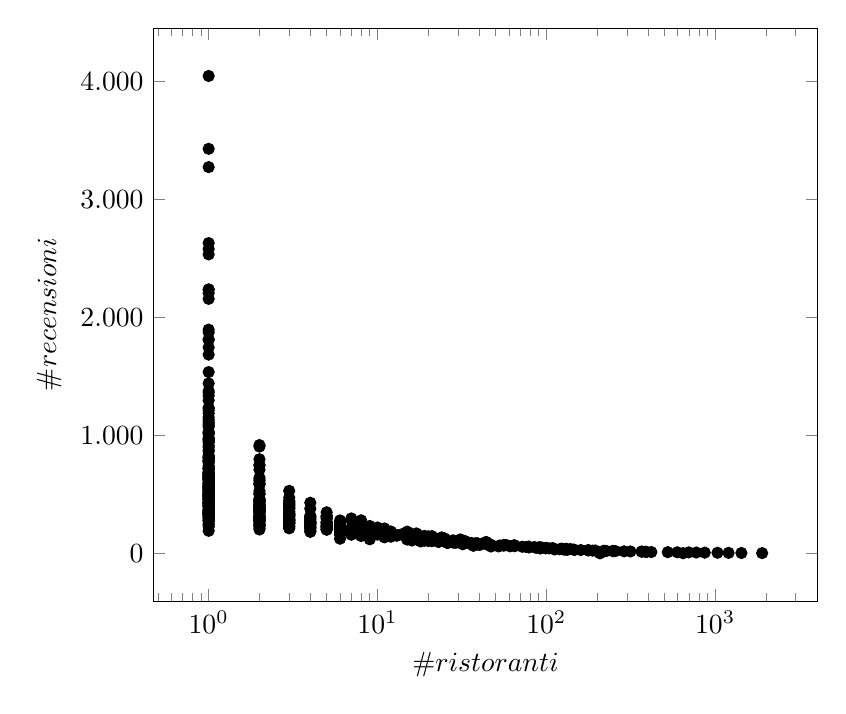
\begin{tikzpicture}
\begin{axis}[scale=1,xlabel=$\#ristoranti$,ylabel=$\#recensioni$, legend pos=outer north east, xmode=log,
scale only axis]
\addplot[
%        smooth,
		only marks,
        mark=*,
        black
      ] plot coordinates
{
(1, 669) (1, 667) (1, 666) (1, 661) (1, 660) (1, 692) (1, 818) (1, 345) (1, 347) (1, 340) (1, 341) (1, 544) (1, 343) (1, 810) (1, 548) (1, 348) (1, 816) (1, 717) (1, 3276) (1, 713) (1, 1027) (1, 1188) (1, 1747) (1, 424) (1, 414) (1, 411) (1, 290) (1, 590) (1, 593) (1, 318) (1, 1088) (1, 274) (1, 276) (1, 832) (1, 526) (1, 725) (1, 520) (1, 368) (1, 369) (1, 599) (1, 362) (1, 363) (1, 360) (1, 1013) (1, 1235) (1, 1338) (1, 1232) (1, 445) (1, 785) (1, 783) (1, 641) (1, 642) (1, 437) (1, 435) (1, 432) (1, 431) (1, 308) (1, 338) (1, 335) (1, 331) (1, 330) (1, 575) (1, 1073) (1, 252) (1, 629) (1, 499) (1, 2208) (1, 541) (1, 1021) (1, 503) (1, 500) (1, 547) (1, 630) (1, 1213) (1, 634) (1, 2582) (1, 464) (1, 467) (1, 461) (1, 460) (1, 463) (1, 462) (1, 960) (1, 815) (1, 559) (1, 558) (1, 746) (1, 553) (1, 789) (1, 1815) (1, 1811) (1, 878) (1, 3431) (1, 968) (1, 898) (1, 613) (1, 646) (1, 949) (1, 689) (1, 352) (1, 684) (1, 686) (1, 2536) (1, 683) (1, 804) (1, 489) (1, 494) (1, 495) (1, 490) (1, 492) (1, 493) (1, 407) (1, 406) (1, 938) (1, 400) (1, 1378) (1, 282) (1, 2159) (1, 628) (1, 1155) (1, 675) (1, 676) (1, 1099) (1, 576) (1, 1031) (1, 378) (1, 532) (1, 982) (1, 393) (1, 397) (1, 395) (1, 537) (1, 791) (1, 2632) (1, 4049) (1, 428) (1, 534) (1, 422) (1, 425) (1, 913) (1, 426) (1, 582) (1, 580) (1, 1133) (1, 302) (1, 413) (1, 305) (1, 589) (1, 241) (1, 1298) (1, 639) (1, 498) (1, 511) (1, 513) (1, 512) (1, 517) (1, 621) (1, 627) (1, 624) (1, 452) (1, 455) (1, 1875) (1, 484) (1, 970) (1, 658) (1, 659) (1, 569) (1, 650) (1, 562) (1, 651) (1, 564) (1, 480) (1, 226) (1, 192) (1, 865) (1, 723) (1, 501) (1, 728) (1, 601) (1, 1898) (1, 657) (1, 1442) (1, 1538) (1, 326) (1, 324) (1, 1114) (1, 329) (1, 1363) (1, 475) (1, 778) (1, 655) (1, 485) (1, 567) (1, 482) (1, 2239) (1, 2237) (1, 477) (1, 1686) (1, 358) (1, 770) (2, 346) (2, 595) (2, 710) (2, 364) (2, 365) (2, 410) (2, 298) (2, 295) (2, 293) (2, 291) (2, 271) (2, 275) (2, 278) (2, 313) (2, 300) (2, 367) (2, 366) (2, 448) (2, 444) (2, 385) (2, 386) (2, 387) (2, 906) (2, 643) (2, 439) (2, 433) (2, 339) (2, 744) (2, 250) (2, 505) (2, 502) (2, 465) (2, 919) (2, 239) (2, 230) (2, 615) (2, 357) (2, 355) (2, 350) (2, 214) (2, 401) (2, 409) (2, 286) (2, 267) (2, 399) (2, 530) (2, 371) (2, 373) (2, 376) (2, 303) (2, 799) (2, 420) (2, 586) (2, 309) (2, 585) (2, 304) (2, 244) (2, 243) (2, 419) (2, 626) (2, 453) (2, 454) (2, 311) (2, 316) (2, 752) (2, 394) (2, 325) (2, 203) (2, 509) (2, 319) (3, 292) (3, 270) (3, 277) (3, 279) (3, 441) (3, 447) (3, 384) (3, 434) (3, 334) (3, 337) (3, 336) (3, 254) (3, 255) (3, 288) (3, 314) (3, 287) (3, 235) (3, 356) (3, 351) (3, 213) (3, 218) (3, 284) (3, 403) (3, 283) (3, 263) (3, 260) (3, 258) (3, 379) (3, 531) (3, 377) (3, 392) (3, 396) (3, 253) (3, 423) (3, 412) (3, 306) (3, 418) (3, 317) (3, 228) (3, 323) (3, 327) (3, 328) (3, 474) (4, 294) (4, 190) (4, 193) (4, 272) (4, 273) (4, 380) (4, 430) (4, 251) (4, 237) (4, 307) (4, 217) (4, 211) (4, 262) (4, 261) (4, 266) (4, 259) (4, 289) (4, 247) (4, 248) (4, 224) (4, 183) (4, 310) (4, 223) (4, 322) (5, 349) (5, 299) (5, 296) (5, 312) (5, 256) (5, 234) (5, 232) (5, 264) (5, 268) (5, 257) (5, 242) (5, 315) (5, 227) (5, 225) (5, 222) (5, 320) (5, 201) (5, 205) (5, 204) (5, 207) (6, 167) (6, 161) (6, 125) (6, 191) (6, 280) (6, 238) (6, 231) (6, 210) (6, 219) (6, 265) (6, 246) (6, 182) (6, 221) (6, 200) (6, 202) (6, 208) (7, 297) (7, 197) (7, 215) (7, 285) (7, 175) (7, 172) (7, 189) (7, 159) (8, 196) (8, 169) (8, 236) (8, 148) (8, 281) (8, 269) (8, 245) (8, 240) (8, 249) (8, 176) (8, 188) (8, 229) (8, 206) (8, 209) (9, 165) (9, 120) (9, 198) (9, 194) (9, 233) (9, 144) (9, 216) (9, 139) (9, 162) (9, 174) (9, 173) (9, 171) (9, 180) (10, 166) (10, 160) (10, 199) (10, 195) (10, 177) (10, 181) (10, 220) (11, 168) (11, 140) (11, 212) (11, 137) (11, 179) (11, 178) (11, 187) (11, 150) (12, 156) (12, 142) (12, 186) (12, 184) (12, 157) (13, 155) (13, 154) (13, 151) (13, 153) (14, 164) (14, 158) (15, 121) (15, 143) (15, 118) (15, 185) (16, 163) (16, 110) (16, 152) (17, 141) (17, 133) (17, 134) (17, 170) (18, 102) (18, 146) (18, 138) (19, 115) (19, 128) (19, 108) (19, 130) (19, 135) (19, 149) (20, 106) (20, 145) (20, 129) (20, 117) (21, 104) (21, 112) (21, 147) (21, 131) (21, 116) (21, 113) (22, 123) (23, 114) (23, 97) (24, 122) (24, 124) (24, 126) (24, 109) (24, 132) (24, 136) (25, 127) (25, 103) (26, 99) (26, 95) (26, 88) (28, 92) (28, 111) (29, 90) (29, 93) (30, 100) (30, 107) (31, 94) (31, 119) (32, 101) (32, 91) (32, 96) (32, 83) (32, 78) (33, 105) (35, 85) (36, 89) (36, 82) (37, 65) (37, 70) (38, 86) (38, 75) (39, 81) (39, 87) (40, 72) (41, 80) (41, 77) (44, 98) (44, 79) (45, 84) (46, 76) (47, 59) (47, 74) (52, 60) (53, 64) (53, 67) (56, 66) (56, 73) (58, 71) (61, 61) (61, 63) (64, 68) (65, 69) (65, 62) (72, 57) (76, 55) (78, 56) (79, 58) (79, 51) (85, 54) (87, 48) (91, 53) (91, 52) (92, 49) (92, 42) (94, 50) (99, 44) (99, 45) (100, 47) (104, 43) (109, 46) (110, 40) (112, 34) (120, 36) (123, 41) (126, 35) (129, 32) (130, 38) (132, 39) (133, 31) (139, 37) (145, 33) (147, 30) (160, 29) (177, 26) (177, 28) (178, 27) (188, 24) (195, 25) (208, 1) (219, 23) (227, 21) (248, 22) (249, 19) (257, 20) (289, 18) (315, 17) (367, 15) (367, 16) (386, 14) (393, 13) (419, 12) (524, 11) (597, 10) (646, 2) (698, 9) (773, 8) (868, 7) (1033, 6) (1201, 5) (1431, 4) (1899, 3)
};

\legend{}
\end{axis}
\end{tikzpicture}
\caption{Il grafico mostra il numero di recensioni rispetto al numero di ristoranti}
\end{figure}

\begin{figure}[H]
\centering
\includegraphics[scale=0.8]{adessoDecido2}
\caption{utenti-\#review}
\end{figure}

\paragraph*{Movielens} Il movielens è stato usato semplicemente come metodo di confronto dell'algoritmo da noi utilizzato su un dataset più omogeneo.\\
Alcuni dati del dataset Movielens:\\
\begin{itemize}
\item Numero recensioni: 100000
\item Numero utenti: 943\\
di cui ognuno ha almeno 20 review
\item Numero ristoranti: 1682
\end{itemize}

\section*{Collaborative filtering\footnote{\textbf{Collaborative Filtering Recommender Systems}, Michael D. Ekstrand, John T. Riedl and Joseph A. Konstan}}
Il Collaborative filtering è un popolare algoritmo per un reccomender system che basa le sue predizioni e raccomandazioni sui voti, o il comportamento, degli altri utenti nel sistema.\\
Si è quindi creato un funzione di rating prediction sia basata sugli utenti che sui oggetti utilizzando le formule di seguito esposte. Si è poi usato tale predizioni per creare un reccomender system.

\subsection*{Misure utilizzate}
$N$ è il vicinato\\
$s(u, v)$ funzione similarità come sotto\\
$r_{u,i}$ rating user $u$ su oggetto $i$\\
$\bar{r}_u$ media voti utente $u$\\

\paragraph*{Calcolo predizione voto User-User}
\begin{equation}
p_{u,i} = \bar{r}_u + \frac{\sum_{u' \in N} s(u, u')(r_{u', i} - \bar{r}_{u'})}{\sum_{u' \in N} \mid s(u, u')\mid}
\label{predUser1}
\end{equation}
Si è poi provato ad utilizzare anche la seguente formula alternativa:
\begin{equation}
p_{u,i} = \bar{r}_u +\sigma_{u'} \frac{\sum_{u' \in N} s(u, u')(r_{u', i} - \bar{r}_{u'})/\sigma_{u'}}{\sum_{u' \in N} \mid s(u, u')\mid}
\label{predUser2}
\end{equation}

La similarità tra utenti è stata calcolata tramite la correlazione di Pearson
\begin{equation}
s(u,v) = \frac{\sum_{i \in I_u \cap I_v}(r_{u,i}-\bar{r}_u)(r_{v,i} - \bar{r}_v)}{\sqrt{\sum_{i \in I_u \cap I_v}(r_{u,i}-\bar{r}_u)^2} \sqrt{\sum_{i \in I_u \cap I_v}(r_{v,i} - \bar{r}_v)^2}}
\end{equation}

\paragraph*{Calcolo predizione voto Item-Item}
\begin{equation}
p_{u,i} = \frac{\sum_{j \in S}s(i,j)r_{u,j}}{\sum_{j \in S}\mid s(i,j) \mid}
\label{predItem1}
\end{equation}

La similarità tra oggetti è stata calcolata tramite Cosine Similarity
\begin{equation}
s(i,j) = \frac{r_i \cdot r_j}{\parallel r_i \parallel_2 \parallel r_j \parallel_2}
\end{equation}

\paragraph*{Reccomender system} Si è poi usata la seguente formula per effettuare una rating prediction ibrida a partire dai due precedenti metodi
\begin{equation}
\alpha p_{u,i}^U + (1-\alpha) p_{u,i}^I
\end{equation}
In cui $p_{u,i}^U$ è la predizione come da equazione \ref{predUser1} e $p_{u,i}^I$ è la 
predizione come da equazione \ref{predItem1}
\newpage
\section*{Dati sperimentali}
Il dataset, soprattutto lo Yelp, ha subito un preprocessing dei dati per cercare di rendere meno sparsa la matrice, di seguito i dati relativi al dataset a cui sono stati rimossi tutti gli utenti con meno di 100 recensioni:\\
Media recensioni ad utente: 166.286353468\\
Minimo: 101 Massimo: 596\\
Percentile 25\% 112.5\\
Percentile 75\% 184.0\\
Mediana 137.0\\

% ------------------------------------------------------------

Nei grafici seguenti vengono riportate le percentuali di true positive (TP) ricavate dai test effettuati sui due diversi dataset, al variare di $\alpha$.\\
L'algoritmo denominato ''MIO'' ha un $\alpha$ ricavato dalla formula in equazione \ref{alphamio}, che come si può notare non riesce a mantenere una buona media per il dataset Yelp, ma viceversa si comporta molto bene per il movielens.\\

\begin{equation}
\alpha = \frac{1}{10} \cdot \frac{1}{2}^{\frac{|TestSet|}{1000}}
\label{alphamio}
\end{equation}

Per effettuare i test è stata fatta una cross validation con 5 folds. Quindi la percentuale di TP è la media dei 5.

\begin{figure}[H]
\begin{minipage}{.4\textwidth}
  
  	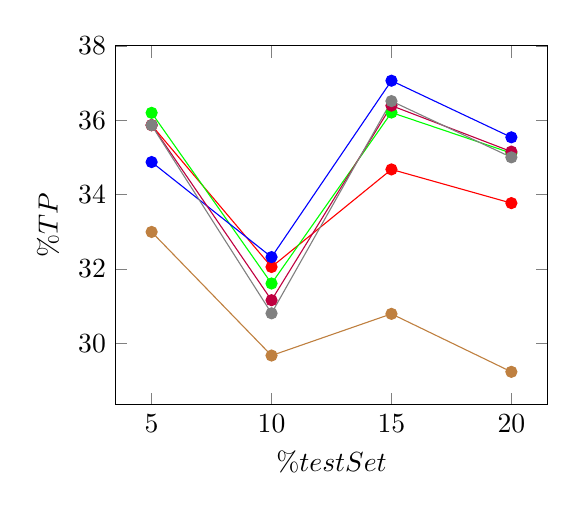
\begin{tikzpicture}
	\begin{axis}[scale=0.8,xlabel=$\% testSet$,ylabel=$\% TP$, legend pos=outer north east, ymax = 38]
\addplot[ %alpha = 0
%        smooth,
        mark=*,
        brown
      ] plot coordinates
{
 (5, 32.9939)(10, 29.6698)(15, 30.791)(20, 29.2312)
};
\addplot[ %alpha = 0.2
%        smooth,
        mark=*,
        red
      ] plot coordinates
{
(5, 35.8653)(10, 32.0517)(15, 34.6757)(20, 33.7692) 
};
\addplot[ %alpha = 0.4
%        smooth,
        mark=*,
        green
      ] plot coordinates
{ 
(5, 36.1974)(10, 31.6071)(15, 36.2054)(20, 35.1146) 
};
\addplot[ %alpha = 0.6
%        smooth,
        mark=*,
        blue
      ] plot coordinates
{
(5, 34.8736)(10, 32.3171)(15, 37.0618)(20, 35.5385) 
};
\addplot[ %alpha = 0.8
%        smooth,
        mark=*,
        purple
      ] plot coordinates
{
(5, 35.8682)(10, 31.1583)(15, 36.3911)(20, 35.1543) 
};
\addplot[ %alpha = 1
%        smooth,
        mark=*,
        gray
      ] plot coordinates
{
(5, 35.864)(10, 30.8051)(15, 36.5127)(20, 35.0001)
};
\addplot[ %MIO
%        smooth,
        mark=*,
        black
      ] plot coordinates
{

};
%<\legend{$\alpha=0\;(Item)$, $\alpha=0.2$, $\alpha=0.4$, $\alpha=0.6$, $\alpha=0.8$, $\alpha=1\;(User)$, $MIO$ }
\end{axis}
	\end{tikzpicture} 
	
  \captionof{figure}{Eq \ref{predUser1},\ref{predItem1}}
  \label{fig:test1}
\end{minipage}%
\qquad\qquad
\begin{minipage}{.4\textwidth}
  
	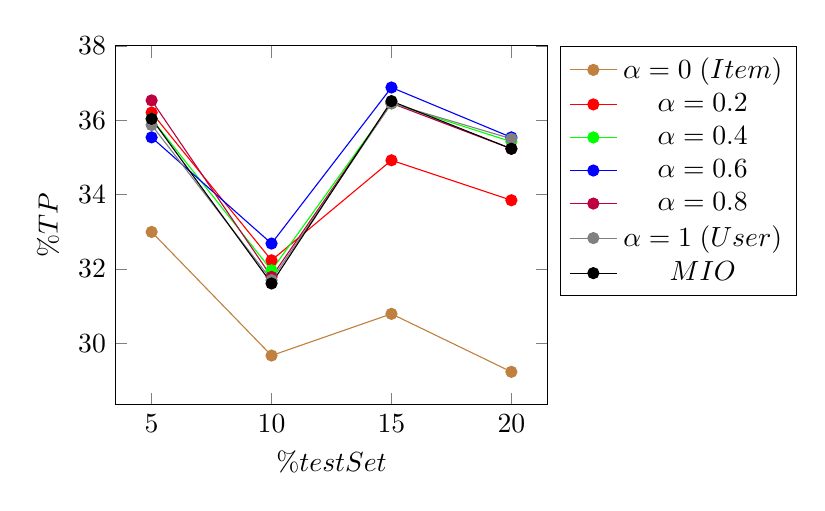
\begin{tikzpicture}
	\begin{axis}[scale=0.8,xlabel=$\% testSet$,ylabel=$\% TP$, legend pos=outer north east, ymax = 38]
\addplot[ %alpha = 0
%        smooth,
        mark=*,
        brown
      ] plot coordinates
{
(5, 32.9939)(10, 29.6698)(15, 30.791)(20, 29.2312) 
};
\addplot[ %alpha = 0.2
%        smooth,
        mark=*,
        red
      ] plot coordinates
{
(5, 36.2042)(10, 32.2311)(15, 34.9213)(20, 33.8458) 
};
\addplot[ %alpha = 0.4
%        smooth,
        mark=*,
        green
      ] plot coordinates
{
(5, 36.0361)(10, 31.9607)(15, 36.4523)(20, 35.4221) 
};
\addplot[ %alpha = 0.6
%        smooth,
        mark=*,
        blue
      ] plot coordinates
{
(5, 35.5375)(10, 32.6818)(15, 36.8797)(20, 35.5375) 
};
\addplot[ %alpha = 0.8
%        smooth,
        mark=*,
        purple
      ] plot coordinates
{
(5, 36.5321)(10, 31.7846)(15, 36.4549)(20, 35.2308) 
};
\addplot[ %alpha = 1
%        smooth,
        mark=*,
        gray
      ] plot coordinates
{
(5, 35.8696)(10, 31.698)(15, 36.4528)(20, 35.5009)
};
\addplot[ %MIO
%        smooth,
        mark=*,
        black
      ] plot coordinates
{
(5, 36.0362) (10, 31.6079)(15, 36.5123)(20, 35.2314) 
};
\legend{$\alpha=0\;(Item)$, $\alpha=0.2$, $\alpha=0.4$, $\alpha=0.6$, $\alpha=0.8$, $\alpha=1\;(User)$, $MIO$ }
\end{axis}
	\end{tikzpicture}  
  
  \captionof{figure}{Eq \ref{predUser2},\ref{predItem1}}
  \label{fig:test2}
\end{minipage}
\caption{yelp tagliato a 100}
\end{figure}

% -----------------------------------------------------------


\begin{figure}[H]
\begin{minipage}{.4\textwidth}
  
  	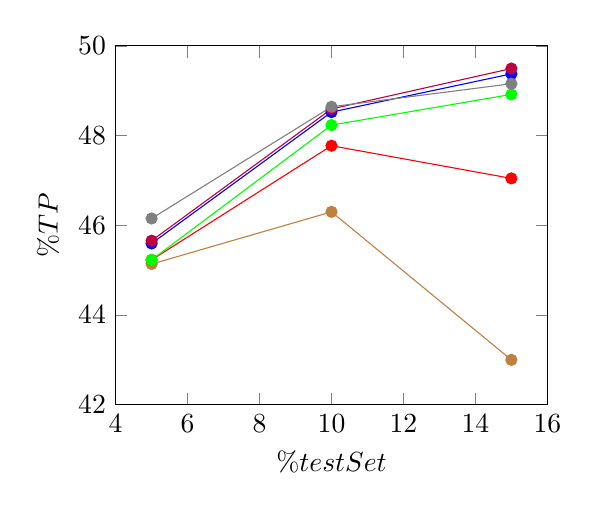
\begin{tikzpicture}
	\begin{axis}[scale=0.8,xlabel=$\% testSet$,ylabel=$\% TP$, legend pos=outer north east, ymax = 50, ymin = 42]
\addplot[ %alpha = 0
%        smooth,
        mark=*,
        brown
      ] plot coordinates
{
 (5, 45.1316)(10, 46.2959)(15, 42.9938)
};
\addplot[ %alpha = 0.2
%        smooth,
        mark=*,
        red
      ] plot coordinates
{
(5, 45.2246) (10, 47.7711)(15, 47.0427)
};
\addplot[ %alpha = 0.4
%        smooth,
        mark=*,
        green
      ] plot coordinates
{
(5, 45.2253)(10, 48.2312)(15, 48.9162)
};
\addplot[ %alpha = 0.6
%        smooth,
        mark=*,
        blue
      ] plot coordinates
{
 (5, 45.5908)(10, 48.5211) (15, 49.374)
};
\addplot[ %alpha = 0.8
%        smooth,
        mark=*,
        purple
      ] plot coordinates
{
(5, 45.653)(10, 48.5925)(15, 49.493)
};
\addplot[ %alpha = 1
%        smooth,
        mark=*,
        gray
      ] plot coordinates
{
(5, 46.148) (10, 48.6405)(15, 49.1537)
};
\addplot[ %MIO
%        smooth,
        mark=*,
        yellow
      ] plot coordinates
{

};
%<\legend{$\alpha=0\;(Item)$, $\alpha=0.2$, $\alpha=0.4$, $\alpha=0.6$, $\alpha=0.8$, $\alpha=1\;(User)$, $MIO$ }
\end{axis}
	\end{tikzpicture} 
	
  \captionof{figure}{Eq \ref{predUser1},\ref{predItem1}}
  \label{fig:test1}
\end{minipage}%
\qquad\qquad
\begin{minipage}{.4\textwidth}
  
	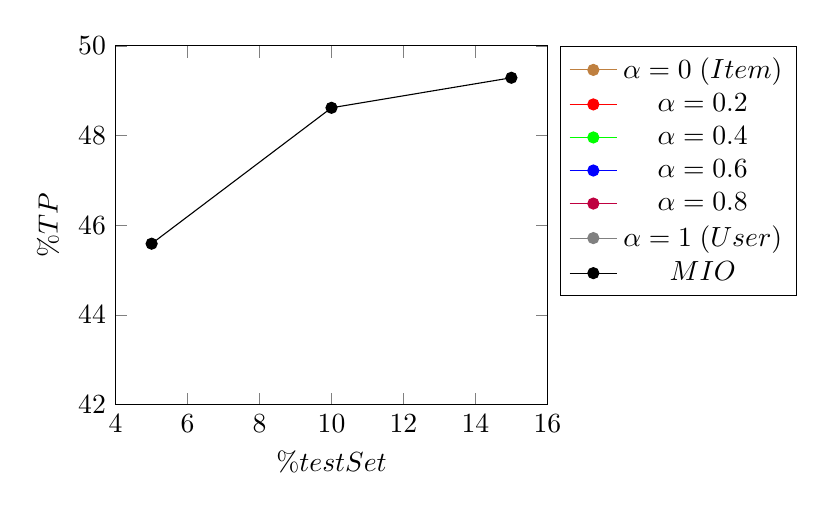
\begin{tikzpicture}
	\begin{axis}[scale=0.8,xlabel=$\% testSet$,ylabel=$\% TP$, legend pos=outer north east, ymax = 50, ymin = 42]
\addplot[ %alpha = 0
%        smooth,
        mark=*,
        brown
      ] plot coordinates
{
(5,0)
};
\addplot[ %alpha = 0.2
%        smooth,
        mark=*,
        red
      ] plot coordinates
{
(5,0)
};
\addplot[ %alpha = 0.4
%        smooth,
        mark=*,
        green
      ] plot coordinates
{
(5,0)
};
\addplot[ %alpha = 0.6
%        smooth,
        mark=*,
        blue
      ] plot coordinates
{
(5,0)
};
\addplot[ %alpha = 0.8
%        smooth,
        mark=*,
        purple
      ] plot coordinates
{
(5,0)
};
\addplot[ %alpha = 1
%        smooth,
        mark=*,
        gray
      ] plot coordinates
{
(5,0)
};
\addplot[ %MIO
%        smooth,
        mark=*,
        black
      ] plot coordinates
{
(5, 45.5853)(10, 48.6167)(15, 49.2869)
};
\legend{$\alpha=0\;(Item)$, $\alpha=0.2$, $\alpha=0.4$, $\alpha=0.6$, $\alpha=0.8$, $\alpha=1\;(User)$, $MIO$ }
\end{axis}
	\end{tikzpicture}  
  
  \captionof{figure}{Eq \ref{predUser2},\ref{predItem1}}
  \label{fig:test2}
\end{minipage}
\caption{yelp tagliato a 50}
\end{figure}

% -----------------------------------------------------------

\begin{figure}[H]
\begin{minipage}{.4\textwidth}
  
  	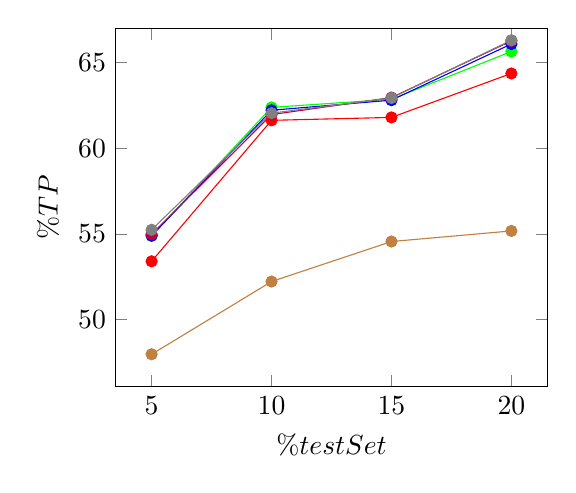
\begin{tikzpicture}
	\begin{axis}[scale=0.8,xlabel=$\% testSet$,ylabel=$\% TP$, legend pos=outer north east, ymax = 67]
\addplot[ %alpha = 0
%        smooth,
        mark=*,
        brown
      ] plot coordinates
{
(5, 47.9874)(10, 52.2271)(15, 54.5617)(20, 55.1799) 
};
\addplot[ %alpha = 0.2
%        smooth,
        mark=*,
        red
      ] plot coordinates
{
(5, 53.4081)(10, 61.6285)(15, 61.8002)(20, 64.3635) 
};
\addplot[ %alpha = 0.4
%        smooth,
        mark=*,
        green
      ] plot coordinates
{
 (5, 54.9028)(10, 62.3839)(15, 62.8559)(20, 65.642) 
};
\addplot[ %alpha = 0.6
%        smooth,
        mark=*,
        blue
      ] plot coordinates
{
(5, 54.8982)(10, 62.2158)(15, 62.8056)(20, 66.0806) 
};
\addplot[ %alpha = 0.8
%        smooth,
        mark=*,
        purple
      ] plot coordinates
{
(5, 54.9855)(10, 61.9641)(15, 62.9562)(20, 66.2604) 
};
\addplot[ %alpha = 1
%        smooth,
        mark=*,
        gray
      ] plot coordinates
{
(5, 55.2456)(10, 62.0479)(15, 62.931)(20, 66.3005) 
};
\addplot[ %MIO
%        smooth,
        mark=*,
        yellow
      ] plot coordinates
{

};
%<\legend{$\alpha=0\;(Item)$, $\alpha=0.2$, $\alpha=0.4$, $\alpha=0.6$, $\alpha=0.8$, $\alpha=1\;(User)$, $MIO$ }
\end{axis}
	\end{tikzpicture} 
	
  \captionof{figure}{Eq \ref{predUser1},\ref{predItem1}}
  \label{fig:test1}
\end{minipage}%
\qquad\qquad
\begin{minipage}{.4\textwidth}
  
	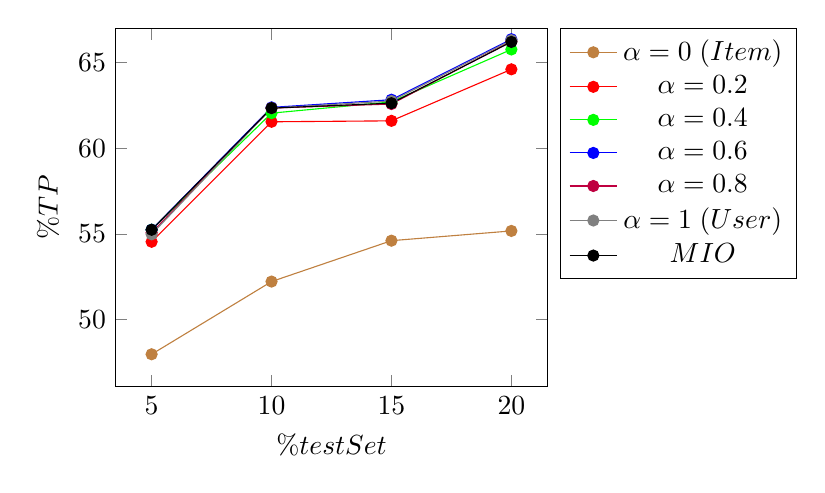
\begin{tikzpicture}
	\begin{axis}[scale=0.8,xlabel=$\% testSet$,ylabel=$\% TP$, legend pos=outer north east, ymax = 67]
\addplot[ %alpha = 0
%        smooth,
        mark=*,
        brown
      ] plot coordinates
{
(5, 47.9874)(10, 52.2271)(15, 54.612)(20, 55.1799) 
};
\addplot[ %alpha = 0.2
%        smooth,
        mark=*,
        red
      ] plot coordinates
{
(5, 54.547)(10, 61.5441)(15, 61.5995)(20, 64.6036) 
};
\addplot[ %alpha = 0.4
%        smooth,
        mark=*,
        green
      ] plot coordinates
{
(5, 55.2518)(10, 62.0477)(15, 62.7054)(20, 65.7615) 
};
\addplot[ %alpha = 0.6
%        smooth,
        mark=*,
        blue
      ] plot coordinates
{ 
(5, 55.2499)(10, 62.3842)(15, 62.831)(20, 66.3609) 
};
\addplot[ %alpha = 0.8
%        smooth,
        mark=*,
        purple
      ] plot coordinates
{ 
(5, 55.0733)(10, 62.3419)(15, 62.5794)(20, 66.241) 
};
\addplot[ %alpha = 1
%        smooth,
        mark=*,
        gray
      ] plot coordinates
{
(5, 54.9836)(10, 62.3419)(15, 62.7553)(20, 66.301)
};
\addplot[ %MIO
%        smooth,
        mark=*,
        black
      ] plot coordinates
{
(5, 55.2464)(10, 62.3419)(15, 62.6296) (20, 66.2009)
};
\legend{$\alpha=0\;(Item)$, $\alpha=0.2$, $\alpha=0.4$, $\alpha=0.6$, $\alpha=0.8$, $\alpha=1\;(User)$, $MIO$ }
\end{axis}
	\end{tikzpicture}  
  
  \captionof{figure}{Eq \ref{predUser2},\ref{predItem1}}
  \label{fig:test2}
\end{minipage}
\caption{movie100k normale}
\end{figure}

% -----------------------------------------------------------

\begin{figure}[H]
\begin{minipage}{.4\textwidth}
  
  	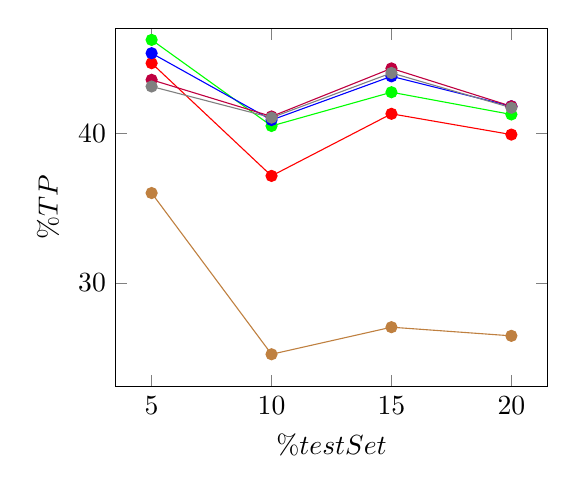
\begin{tikzpicture}
	\begin{axis}[scale=0.8,xlabel=$\% testSet$,ylabel=$\% TP$, legend pos=outer north east, ymax = 47]
\addplot[ %alpha = 0
%        smooth,
        mark=*,
        brown
      ] plot coordinates
{
(5, 36) (10, 25.2381)(15, 27.0455)(20, 26.4677)
};
\addplot[ %alpha = 0.2
%        smooth,
        mark=*,
        red
      ] plot coordinates
{
(5, 44.6667)(10, 37.1429)(15, 41.2879)(20, 39.9005) 
};
\addplot[ %alpha = 0.4
%        smooth,
        mark=*,
        green
      ] plot coordinates
{
(5, 46.2222)(10, 40.4762)(15, 42.7273) (20, 41.2438)
};
\addplot[ %alpha = 0.6
%        smooth,
        mark=*,
        blue
      ] plot coordinates
{
(5, 45.3333)(10, 40.873)(15, 43.7879) (20, 41.791)
};
\addplot[ %alpha = 0.8
%        smooth,
        mark=*,
        purple
      ] plot coordinates
{
(5, 43.5556)(10, 41.1111)(15, 44.3182) (20, 41.791)
};
\addplot[ %alpha = 1
%        smooth,
        mark=*,
        gray
      ] plot coordinates
{
(5, 43.1111)(10, 41.0317)(15, 44.0152) (20, 41.6915)

};
\addplot[ %MIO
%        smooth,
        mark=*,
        yellow
      ] plot coordinates
{

};
%<\legend{$\alpha=0\;(Item)$, $\alpha=0.2$, $\alpha=0.4$, $\alpha=0.6$, $\alpha=0.8$, $\alpha=1\;(User)$, $MIO$ }
\end{axis}
	\end{tikzpicture} 
	
  \captionof{figure}{Eq \ref{predUser1},\ref{predItem1}}
  \label{fig:test1}
\end{minipage}%
\qquad\qquad
\begin{minipage}{.4\textwidth}
  
	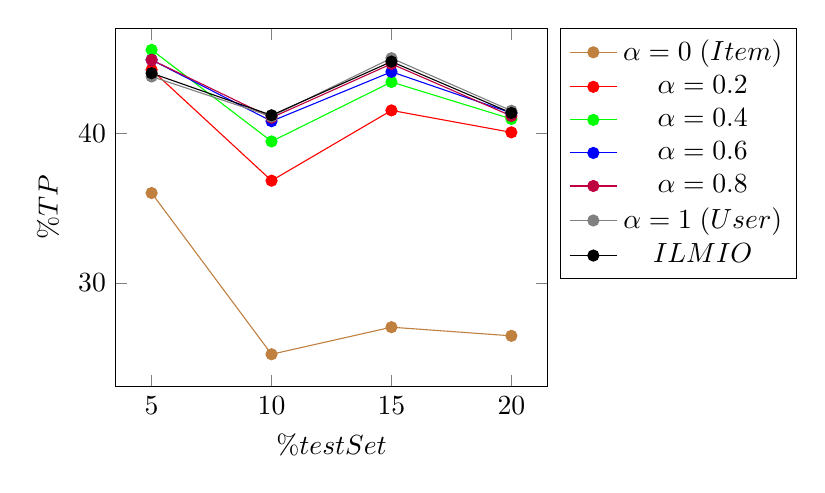
\begin{tikzpicture}
	\begin{axis}[scale=0.8,xlabel=$\% testSet$,ylabel=$\% TP$, legend pos=outer north east, ymax = 47]
\addplot[ %alpha = 0
%        smooth,
        mark=*,
        brown
      ] plot coordinates
{
(5, 36) (10, 25.2381)(15, 27.0455)(20, 26.4677)
};
\addplot[ %alpha = 0.2
%        smooth,
        mark=*,
        red
      ] plot coordinates
{
(5, 44.2222)(10, 36.8254)(15, 41.5152)(20, 40.0498) 
};
\addplot[ %alpha = 0.4
%        smooth,
        mark=*,
        green
      ] plot coordinates
{
(5, 45.5556)(10, 39.4444)(15, 43.4091)(20, 40.9453) 
};
\addplot[ %alpha = 0.6
%        smooth,
        mark=*,
        blue
      ] plot coordinates
{
(5, 44.8889)(10, 40.7937)(15, 44.0909)(20, 41.3433) 
};
\addplot[ %alpha = 0.8
%        smooth,
        mark=*,
        purple
      ] plot coordinates
{
(5, 44.8889)(10, 41.0317)(15, 44.6212)(20, 41.1443) 
};
\addplot[ %alpha = 1
%        smooth,
        mark=*,
        gray
      ] plot coordinates
{
(5, 43.7778)(10, 41.1111)(15, 45) (20, 41.4925)
};
\addplot[ %MIO
%        smooth,
        mark=*,
        black
      ] plot coordinates
{
(5, 44)(10, 41.1905)(15, 44.7727)(20, 41.3433)
};
\legend{$\alpha=0\;(Item)$, $\alpha=0.2$, $\alpha=0.4$, $\alpha=0.6$, $\alpha=0.8$, $\alpha=1\;(User)$, $ILMIO$ }
\end{axis}
	\end{tikzpicture}  
  
  \captionof{figure}{Eq \ref{predUser2},\ref{predItem1}}
  \label{fig:test2}
\end{minipage}
\caption{movie100k tagliato 100}
\end{figure}

\subsection*{Rating Prediction}
Di seguito si riportano alcuni dati rilevati dalla rating prediction

\begin{table}[H]
\caption{\#review minimo:100, ibrida con $\alpha= 0.4$}
\begin{tabular}{llllll}
TestSet & RMSE  & NRMSE & MAE & NMAE &  \\ 
5\% & 0.958719 & 0.23968 & 0.714333  & 0.178583 & user\\
5\% & 1.17647 & 0.294117 & 0.922233  & 0.230558 & item\\ \hline
5\% & 0.952556 & 0.238139 & 0.72481& 0.181202 & ibrida \\ \hline
10\% & 1.08807 & 0.272016 & 0.860282 & 0.21507& user \\
10\% & 0.917415 & 0.229354 & 0.7091 & 0.177275& item \\ \hline
10\% & 0.911735 & 0.227934 & 0.712978 & 0.178244& ibrida \\ \hline
15\% & 1.06429& 0.266071& 0.843278& 0.210819 & user \\ 
15\% & 0.947033& 0.236758& 0.74401& 0.186002 & item \\ \hline
15\% & 0.919638& 0.229909& 0.730029& 0.182507 & ibrida \\ \hline
20\% & 1.0829& 0.270725& 0.84769& 0.211923 & user\\
20\% & 0.928202& 0.232051& 0.716904& 0.179226 & item\\ \hline
20\% & 0.921181& 0.230295& 0.716425& 0.179106 & ibrida\\
\end{tabular}
\label{table:minimo100-sceltaCasuale}
\end{table}

\begin{figure}[H]
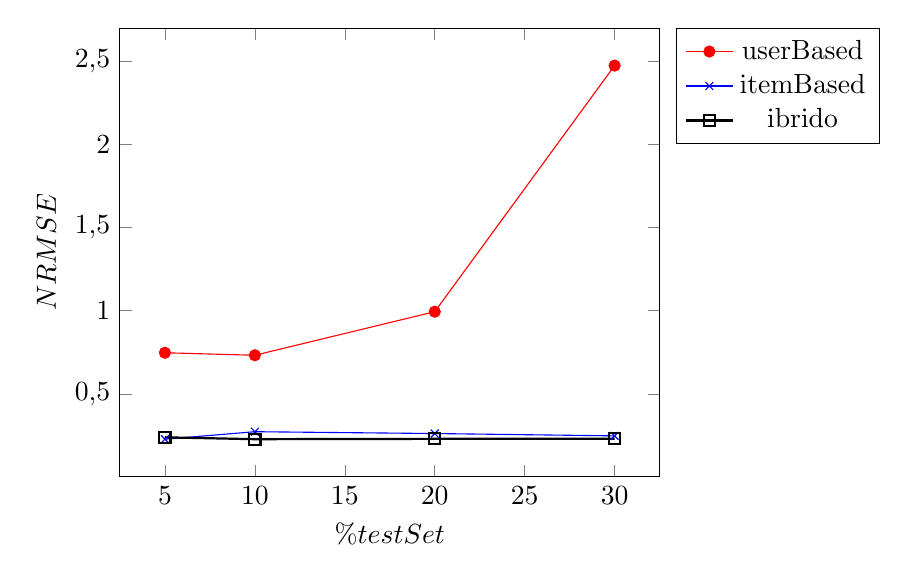
\begin{tikzpicture}
\begin{axis}[scale=1,xlabel=$\% testSet$,ylabel=$NRMSE$, legend pos=outer north east]
\addplot[
%        smooth,
        mark=*,
        red
      ] plot coordinates
{
(5, 0.747) (10, 0.732) (20,  0.994) (30, 2.475)
};
\addplot[
%        smooth,
        mark=x,
        blue
      ] plot coordinates
{
(5, 0.227) (10, 0.272) (20, 0.261) (30,  0.247)
};
\addplot[
        thick,
        mark=square,
        black
      ] plot coordinates
{
(5, 0.2381) (10, 0.227) (20, 0.229) (30,  0.230)
};
\legend{userBased, itemBased, ibrido}
\end{axis}
\end{tikzpicture}
\caption{tabella \ref{table:minimo100-sceltaCasuale}}
\end{figure}
\newpage
\subsection*{Il codice}
Il codice è stato scritto in c++ utilizzando come strutture dati basi le \\
\href{http://www.cplusplus.com/reference/unordered_map/unordered_map/}{unordered\_map}\\
Di seguito si cercherà di dare una spiegazione più esplicativa possibile del codice.\\

Il codice è diviso in 6 file principali:
\begin{itemize}
\item \textbf{main.cpp: } il main ha l'unica funzione di richiamare la funzione \textit{creazioneTestSet} (che si trova nel file \textit{CreateTestSet.cpp}) con i parametri richiesti per la computazione.
\item \textbf{createTestSet.cpp: } contiene la funzione di creazione del test set e il richiamo alle varie funzioni utili all'algoritmo che porteranno al risultato (spiegate poi)
\item \textbf{matrixItem.cpp e matrixUser.cpp:  } sono le funzioni che devono calcolare le matrici di similarità, rispettivamente per utente e oggetto
\item \textbf{ratingPrediction.cpp: } ha il compito di calcolare le varie predizioni (per tutte le tipologie: user, item, ibrida)
\item \textbf{reccomender.cpp: } ha il compito di estrarre le predizioni da raccomandare e controllare effettivamente la buona riuscita di queste
\end{itemize}

\paragraph*{createTestSet.cpp} La sua funzione principale come detto è \textit{creazioneTestSet} che ha una divisione in fasi, crea il test set (scelto in maniera casuale) e per ogni utente poi crea le fold, ne sceglie una da eliminare e richiama quindi la funzione \textit{reccomenderRatingPredictionBased} che avrà il compito di svolgere effettivamente l'algoritmo.
In sequenza questo provvederà a richiamare varie funzioni e quindi creare: la matrice di similarità per utente e per oggetto, calcolare le predizioni e infine avviare il reccomender.

Le fasi di questo metodo sono le seguenti
\begin{itemize}
\item \textit{creazioneMatriceUser} è una semplice coppia di for che scorrono tutta la matrice per riempirla tramite le formule sopra riportate
\item \textit{creazioneMatriceItem} l'idea è la stessa della matrice user, solo che si devono scorrere i bussiness e cambia la formula per calcolare la similarità
\item \textit{calcoloRatingPrediction} questa funzione ha il compito di riempire le hashtable \textit{predizioniUser} e \textit{predizioniItem}. Si è cercato di ottimizzare la funzione scorrendo un unica volta gli utenti, quindi, per ogni utente si calcola separatamente la predizione rispetto agli oggetti e rispetto agli utenti.
\item \textit{ratingPredictionHybrid} semplicemente scorre le predizioni fatte tramite user, le cerca tra i bussiness e le unisce rispetto ad $\alpha$ sull'hash table ibrida
\item \textit{reccomender} è infine l'ultima funzione ad essere richiamata che ha il compito di estrarre, per ogni utente, le predizioni con voto più alto. Queste saranno poi poi da raccomandare. Nella seconda parte della funzione si calcolano quindi i TP e FP comparando i bussiness raccomandati con quelli effettivamente tolti dal test set
\end{itemize}

Il codice debitamente commentato è possibile trovarlo qui\\
\href{https://github.com/sfcoding-school/CollaborativeFilteringHybrid}{GitHub:CollaborativeFilteringHybrid}

\end{document}
